\chapter{Tiempo propio, dilatación temporal y contracción de la longitud}

A menudo elegiremos unidades en las que la velocidad de la luz sea $c=1$. En esas unidades, un año de tiempo y un año luz de distancia pueden compararse directamente, y las fórmulas son mucho más fáciles de leer. Siempre que $c$ tenga importancia física, volveremos a incluirlo. Basta con el análisis dimensional para determinar dónde va.

\section{La cuadrícula galileana del espacio-tiempo}

Comencemos con la relación anterior a Einstein entre un sistema en reposo y un tren que se mueve con velocidad $v$ a lo largo del eje $x$:
\begin{align}
x' &= x-vt, & t'&=t.
\label{eq:l4-galilean}
\end{align}
La segunda ecuación contiene la hipótesis newtoniana del tiempo universal. Todos los observadores usan las mismas superficies de simultaneidad, aunque sus orígenes espaciales se muevan unos respecto de otros.

Supongamos que el observador sin primas está junto a las vías y que el observador con primas viaja en el tren. El origen del tren tiene $x'=0$, así que su línea de universo en las coordenadas sin primas es
\begin{equation}
x=vt.
\end{equation}
Esa línea inclinada es el eje $t'$. En cambio, $t'=t$ indica que todas las líneas de $t'$ constante son las mismas líneas horizontales que las de $t$ constante.

\begin{figure}[H]
\centering
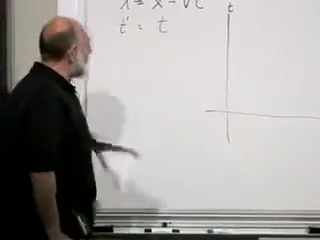
\includegraphics[width=0.72\textwidth]{lecture_04_figure_02.png}
\caption{La transformación galileana y la cuadrícula inicial de $t$-$x$. El origen móvil trazará $x=vt$, mientras los dos sistemas conservan en común las líneas de tiempo constante.}
\lectureframe{00:03:06}
\end{figure}

Al despejar las coordenadas sin primas en la ec.~\eqref{eq:l4-galilean} se obtiene
\begin{align}
x&=x'+vt'=x'+vt, & t&=t'.
\end{align}
La transformación inversa tiene la misma forma, pero con $v$ sustituido por $-v$. Si el tren avanza respecto de la estación, esta se mueve hacia atrás respecto del tren. Esta reciprocidad se conserva en la relatividad especial, pero el tiempo universal no.

\section{La corrección de Lorentz}

Las transformaciones galileanas no pueden hacer que la velocidad de la luz sea la misma en todos los sistemas inerciales. Las relaciones corregidas son, primero, en unidades de $c=1$,
\begin{align}
x'&=\frac{x-vt}{\sqrt{1-v^2}}, &
t'&=\frac{t-vx}{\sqrt{1-v^2}}.
\label{eq:l4-lorentz-natural}
\end{align}
Al volver a las unidades habituales se obtiene
\begin{align}
x'&=\frac{x-vt}{\sqrt{1-v^2/c^2}}, &
t'&=\frac{t-vx/c^2}{\sqrt{1-v^2/c^2}}.
\label{eq:l4-lorentz-c}
\end{align}

\begin{figure}[H]
\centering
\includegraphics[width=0.74\textwidth]{lecture_04_figure_05.png}
\caption{La transformación de Lorentz con los factores de $c$ restituidos.}
\lectureframe{00:09:10}
\end{figure}

Para $v\ll c$, tanto $v^2/c^2$ como $vx/c^2$ son pequeños en las circunstancias en que se usa la mecánica newtoniana. Entonces, la ec.~\eqref{eq:l4-lorentz-c} se reduce al resultado galileano. La relatividad no descarta la cinemática newtoniana; determina el rango en que es válida.

Para $v=c$, el denominador se anula. Un sistema inercial no puede moverse a la velocidad de la luz respecto de otro sistema inercial. Muy por debajo de ese límite las correcciones son pequeñas, pero cerca de él la mezcla de $x$ y $t$ se vuelve inevitable.

El movimiento se eligió a lo largo de $x$, así que las coordenadas transversales no cambian:
\begin{equation}
y'=y,\qquad z'=z.
\end{equation}
Una forma de entender por qué es colocar reglas transversales idénticas en el tren y en el andén. Un observador que se mueve a mitad de camino entre los dos sistemas ve las reglas acercarse con velocidades iguales y opuestas. En la situación no hay nada que pueda hacer que una regla transversal sea más corta que la otra.

\section{Transformaciones de Lorentz a lo largo del cono de luz}

La ec.~\eqref{eq:l4-lorentz-natural} puede interpretarse geométricamente. Sumemos sus dos ecuaciones:
\begin{align}
t'+x'
&=\frac{(t-vx)+(x-vt)}{\sqrt{1-v^2}}\\
&=(t+x)\frac{1-v}{\sqrt{1-v^2}}\\
&=(t+x)\sqrt{\frac{1-v}{1+v}}.
\label{eq:l4-null-plus}
\end{align}
Restémoslas en el orden complementario:
\begin{align}
t'-x'
&=\frac{(t-vx)-(x-vt)}{\sqrt{1-v^2}}\\
&=(t-x)\frac{1+v}{\sqrt{1-v^2}}\\
&=(t-x)\sqrt{\frac{1+v}{1-v}}.
\label{eq:l4-null-minus}
\end{align}

\begin{figure}[H]
\centering
\includegraphics[width=0.75\textwidth]{lecture_04_figure_06.png}
\caption{La transformación de Lorentz expresada mediante las combinaciones nulas $t+x$ y $t-x$. Sus factores de escala son recíprocos.}
\lectureframe{00:18:45}
\end{figure}

Las combinaciones $t+x$ y $t-x$ son coordenadas a lo largo de las dos direcciones $45^\circ$ luminosas. Un impulso de Lorentz comprime una de estas direcciones y estira la otra por el factor inverso. No rota ninguna de ellas fuera de $45^\circ$. Por tanto, los rayos de luz siguen siendo rayos de luz, lo que representa en el espacio-tiempo la invariancia de la velocidad de la luz.

\begin{classroomqa}\audiencequestion{El observador a mitad de camino ve un experimento simétrico, pero ¿cómo demuestra eso el resultado para los observadores del tren y del andén?
\lecturetimestamp{00:20:48}}\lecturerresponse{Se usa además un hecho: la coincidencia de dos sucesos es invariante. Si se encuentran los extremos de las reglas, ese encuentro es un único suceso del espacio-tiempo. Cada observador inercial puede asignarle coordenadas distintas, pero ninguno puede dividir una coincidencia en dos lugares diferentes. Los destellos emitidos donde se encuentran los extremos correspondientes permiten detectar esos sucesos de forma operacional. La simetría del sistema a mitad de camino y la invariancia de las coincidencias entre los dos pares de extremos demuestran que las longitudes transversales son iguales.}
\end{classroomqa}

\begin{classroomqa}\audiencequestion{¿El ciclista que representa el sistema de referencia a mitad de camino debe estar situado físicamente en el punto medio de las reglas?
\lecturetimestamp{00:22:25}}\lecturerresponse{No. Un sistema de referencia es una red completa de observadores y relojes, no un solo ojo en un lugar. El ciclista puede recibir después los destellos de los extremos e inferir dónde se originaron. Lo que importa es la ubicación en el espacio-tiempo de cada suceso de emisión, no dónde se recibe finalmente la luz.}
\end{classroomqa}

La composición de velocidades sucesivas es otra consecuencia de la misma transformación, pero se deja deliberadamente para la próxima clase. La tarea de hoy es identificar la cantidad invariante que mide un reloj en movimiento.

\section{El intervalo invariante}

En una rotación de los ejes cartesianos ordinarios, la cantidad $x^2+y^2$ no cambia. Las transformaciones de Lorentz conservan otra forma cuadrática. A partir de la ec.~\eqref{eq:l4-lorentz-natural},
\begin{align}
t'^2-x'^2
&=\frac{(t-vx)^2-(x-vt)^2}{1-v^2}\\
&=\frac{t^2-2vtx+v^2x^2-x^2+2vtx-v^2t^2}{1-v^2}\\
&=t^2-x^2.
\label{eq:l4-interval}
\end{align}
Los términos mixtos se cancelan y en el numerador restante aparece un factor común $1-v^2$.

\begin{figure}[H]
\centering
\includegraphics[width=0.76\textwidth]{lecture_04_figure_07.png}
\caption{La derivación en la pizarra de $t'^2-x'^2=t^2-x^2$.}
\lectureframe{00:33:15}
\end{figure}

En tres dimensiones espaciales, el invariante es
\begin{equation}
t'^2-x'^2-y'^2-z'^2=t^2-x^2-y^2-z^2
\end{equation}
en unidades de $c=1$. En general, para dos sucesos usamos diferencias de coordenadas:
\begin{equation}
\Delta s^2
=c^2\Delta t^2-\Delta x^2-\Delta y^2-\Delta z^2.
\label{eq:l4-spacetime-interval}
\end{equation}
Todos los observadores inerciales coinciden en este número, aunque discrepen sobre sus términos separados de tiempo y espacio.

\section{Tiempo propio y relojes en movimiento}

Imaginemos una red de observadores en reposo cuyos relojes se han sincronizado intercambiando señales luminosas. Sus lecturas definen el tiempo coordenado $t$. Ahora llevemos un reloj de pulsera a través de esa red. Su propia lectura acompaña al reloj a lo largo de su línea de universo; esa lectura es el tiempo propio.

Para dos sucesos separados temporalmente, definimos
\begin{equation}
c^2\Delta\tau^2
=c^2\Delta t^2-\Delta x^2-\Delta y^2-\Delta z^2.
\label{eq:l4-proper-time}
\end{equation}
En una dimensión espacial y con $c=1$, esto es simplemente
\begin{equation}
\Delta\tau=\sqrt{\Delta t^2-\Delta x^2}.
\end{equation}
La raíz cuadrada es análoga a la fórmula de la distancia ordinaria, pero el signo menos cambia la geometría.

Hay tres casos:
\begin{align}
\Delta t^2-\Delta x^2 &>0 &&\text{timelike},\\
\Delta t^2-\Delta x^2 &=0 &&\text{lightlike},\\
\Delta t^2-\Delta x^2 &<0 &&\text{spacelike}.
\end{align}
Dentro del cono de luz, el tiempo propio es real. Sobre el cono, donde $x=\pm t$, es cero, aunque los sucesos no necesariamente coincidan. Un rayo de luz puede conectar precisamente sucesos así. Fuera del cono, la separación es espacial; es mejor describirla mediante la distancia propia real $\sqrt{\Delta x^2-\Delta t^2}$ que mediante un tiempo de reloj imaginario.

\begin{figure}[H]
\centering
\includegraphics[width=0.73\textwidth]{lecture_04_figure_08.png}

\vspace{0.8em}

\begin{tikzpicture}[x=1.0cm,y=1.0cm]
\draw[->] (-3.3,0) -- (3.3,0) node[right] {$x$};
\draw[->] (0,-0.4) -- (0,4.0) node[above] {$t$};
\draw[thick] (0,0) -- (3.0,3.0) node[above right] {$x=t$};
\draw[thick] (0,0) -- (-3.0,3.0) node[above left] {$x=-t$};
\node at (0,2.0) {timelike};
\node at (2.25,1.05) {spacelike};
\node at (-2.25,1.05) {spacelike};
\end{tikzpicture}\caption{El cono de luz en la pizarra y una clasificación clara de las separaciones temporales, luminosas y espaciales.}
\lectureframe{00:38:40}
\end{figure}

¿Por qué la ec.~\eqref{eq:l4-proper-time} equivale a la lectura de un reloj? Para un reloj en reposo, $\Delta x=0$, así que $\Delta\tau=\Delta t$. Para un reloj que se mueve uniformemente, elijamos el sistema con primas en el que dicho reloj está en reposo. Allí, $\Delta x'=0$, y la invariancia da
\begin{equation}
\Delta\tau
=\sqrt{\Delta t'^2-\Delta x'^2}
=\Delta t'.
\end{equation}
Por tanto, los relojes en movimiento registran el tiempo propio.

\begin{classroomqa}\audiencequestion{¿Se usan «``el intervalo entre los sucesos''» y «``la lectura del reloj''» para referirse a una misma cosa?
\lecturetimestamp{00:44:49}}\lecturerresponse{Coinciden cuando un reloj ideal viaja inercialmente de un suceso al otro. El intervalo invariante es una cantidad geométrica; la diferencia entre las lecturas de los extremos del reloj comóvil es su medición física. Un reloj de coordenadas en reposo generalmente registra un intervalo de tiempo coordenado distinto.}
\end{classroomqa}

\section{Dilatación temporal y simultaneidad}

Consideremos el origen del sistema móvil. Su línea de universo satisface
\begin{equation}
x'=0,\qquad x=vt.
\end{equation}
La misma línea inclinada es tanto la trayectoria del reloj móvil como el eje $t'$.

\begin{figure}[H]
\centering
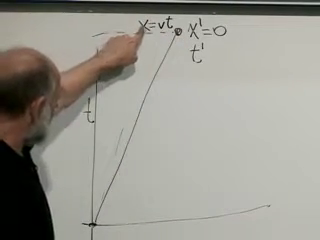
\includegraphics[width=0.72\textwidth]{lecture_04_figure_03.png}
\caption{El origen móvil: $x=vt$, $x'=0$ y el eje $t'$ son tres descripciones de la misma línea de universo.}
\lectureframe{00:48:18}
\end{figure}

Apliquemos el intervalo invariante entre el origen común y un punto posterior de esa línea de universo:
\begin{align}
t'^2-x'^2&=t^2-x^2,\\
t'^2&=t^2-v^2t^2,\\
t'&=t\sqrt{1-v^2}.
\label{eq:l4-time-dilation-natural}
\end{align}
Al restituir $c$,
\begin{equation}
\Delta\tau=\Delta t\sqrt{1-\frac{v^2}{c^2}}
=\frac{\Delta t}{\gamma},
\qquad
\gamma=\frac{1}{\sqrt{1-v^2/c^2}}.
\label{eq:l4-time-dilation}
\end{equation}

\begin{figure}[H]
\centering
\includegraphics[width=0.73\textwidth]{lecture_04_figure_09.png}
\caption{El resultado de la dilatación temporal en la pizarra: el reloj móvil acumula $t'=t\sqrt{1-v^2}$ en unidades con $c=1$.}
\lectureframe{00:50:45}
\end{figure}

El observador en reposo dice que el reloj móvil marcha más despacio. La reciprocidad exige que el observador móvil diga lo mismo de los relojes en reposo. No hay contradicción, porque las dos descripciones comparan pares distintos de sucesos distantes.

En efecto, un valor constante de $t'$ en la ec.~\eqref{eq:l4-lorentz-natural} satisface
\begin{equation}
t-vx=\text{constant}.
\label{eq:l4-simultaneity}
\end{equation}
Las líneas de simultaneidad del observador móvil están inclinadas respecto de las líneas horizontales $t=\text{constant}$. Cada observador considera simultáneas colecciones distintas de lecturas de relojes distantes. Si se tiene presente esta diferencia, la desaceleración recíproca de los relojes resulta coherente.

\begin{figure}[H]
\centering
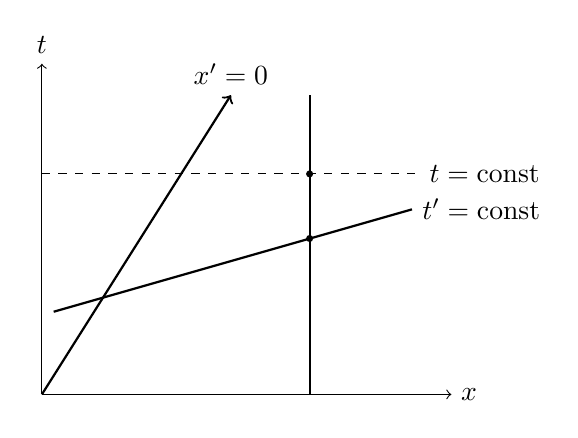
\begin{tikzpicture}[x=1cm,y=1cm]
\draw[->] (0,0) -- (0,4.2) node[above] {$t$};
\draw[->] (0,0) -- (5.2,0) node[right] {$x$};
\draw[thick,->] (0,0) -- (2.4,3.8) node[above] {$x'=0$};
\draw[dashed] (0,2.8) -- (4.8,2.8)
  node[right] {$t=\mathrm{const}$};
\draw[thick] (0.15,1.05) -- (4.7,2.35)
  node[right] {$t'=\mathrm{const}$};
\draw[thick] (3.4,0) -- (3.4,3.8);
\fill (3.4,2.8) circle (0.045);
\fill (3.4,1.98) circle (0.045);
\end{tikzpicture}
\caption{La dilatación temporal recíproca compara lecturas de relojes en distintas superficies de simultaneidad.}
\end{figure}

\section{Las trayectorias de los gemelos}

Dos gemelos parten del mismo suceso. Uno permanece en $x=0$. El otro viaja hacia el exterior a velocidad $v$, invierte el sentido y regresa a la misma velocidad. Cuando se reúnen, comparan todos los procesos físicos que pueden servir como reloj: los relojes de pulsera, los latidos, el metabolismo o el envejecimiento mismo.

Supongamos que cada mitad del viaje dura un tiempo coordenado $T$ en el sistema del gemelo que se queda en casa. Su tiempo propio es
\begin{equation}
\tau_{\mathrm{home}}=2T.
\end{equation}
El suceso de retorno tiene coordenadas $(vT,T)$. Por tanto, el primer tramo del viaje aporta
\begin{align}
\tau_{\mathrm{leg}}
&=\sqrt{T^2-v^2T^2}
=T\sqrt{1-v^2}.
\end{align}
El tramo de regreso aporta la misma cantidad, de modo que
\begin{equation}
\tau_{\mathrm{travel}}=2T\sqrt{1-v^2}<2T.
\label{eq:l4-twin}
\end{equation}

\begin{figure}[H]
\centering
\includegraphics[width=0.73\textwidth]{lecture_04_figure_10.png}

\vspace{0.8em}

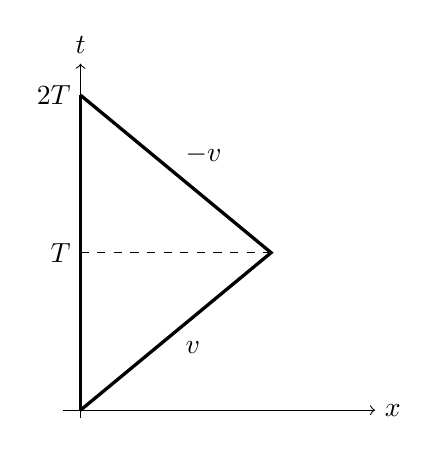
\begin{tikzpicture}[x=1.1cm,y=1cm]
\draw[->] (-0.2,0) -- (3.4,0) node[right] {$x$};
\draw[->] (0,-0.1) -- (0,4.4) node[above] {$t$};
\draw[very thick] (0,0) -- (0,4);
\draw[very thick] (0,0) -- (2.2,2) -- (0,4);
\draw[dashed] (0,2) -- (2.2,2);
\node[left] at (0,2) {$T$};
\node[left] at (0,4) {$2T$};
\node[below right] at (1.1,1.0) {$v$};
\node[above right] at (1.1,3.0) {$-v$};
\end{tikzpicture}\caption{La línea de universo del gemelo que se queda en casa y los dos tramos del viajero. Sus tiempos propios son distintos porque siguen trayectorias diferentes por el espacio-tiempo.}
\lectureframe{00:59:35}
\end{figure}

La diferencia de edad no es contradictoria. La trayectoria del viajero incluye un giro y no está relacionada con la trayectoria recta del gemelo que se queda en casa mediante una única simetría de sistema inercial. En la geometría euclidiana ordinaria, la ruta recta y una ruta quebrada entre dos puntos también tienen longitudes distintas. La geometría de Minkowski invierte cuál de las dos trayectorias tiene el intervalo mayor, pero la comparación sigue siendo geométrica.

\section{Aceleración y reloj ideal}

\begin{classroomqa}\audiencequestion{En el giro la física cambia y el viajero acelera. ¿Eso invalida el cálculo del reloj?
\lecturetimestamp{01:02:19}}\lecturerresponse{La aceleración es real y ayuda a identificar la asimetría; no se debe descartar con argumentos. La esquina pronunciada es solo una idealización gráfica y puede redondearse para representar un giro de duración finita. La hipótesis física adicional es que un reloj suficientemente pequeño y bien construido no se ve afectado por una aceleración moderada y sigue registrando el tiempo propio. Un reloj grande o frágil puede deformarse o romperse, pero eso es un defecto del mecanismo, no del intervalo del espacio-tiempo.}
\end{classroomqa}

Esta hipótesis del reloj ideal no se deduce únicamente de la transformación de Lorentz. Se pone a prueba observando el comportamiento de mecanismos de reloj reales. Un átomo constituye una aproximación mucho mejor que un reloj de cientos de millas de tamaño, porque es más difícil deformar su mecanismo compacto con la aceleración o la gravedad. Mencionar la relatividad general no eliminaría este problema físico: aún habría que saber cómo responde el mecanismo elegido a su entorno.

\begin{classroomqa}\audiencequestion{¿Puede reducirse una trayectoria acelerada a intervalos cortos en los que siga siendo válido el análisis inercial?
\lecturetimestamp{01:09:08}}\lecturerresponse{Sí. Dividamos la curva en segmentos cortos, casi rectos, calculemos el tiempo propio de cada segmento y sumemos los resultados. Es el análogo espacio-temporal de hallar la longitud de una curva ordinaria a partir de muchos segmentos pequeños. En el límite continuo,
\[
\tau=\int \sqrt{1-\frac{v(t)^2}{c^2}}\,dt,
\]
para un movimiento en el espacio-tiempo plano descrito en un sistema de coordenadas inercial.}
\end{classroomqa}

\section{Lo que ven los gemelos}

Las lecturas finales de los relojes pueden determinarse operacionalmente enviando pulsos de luz. Marquemos intervalos de un segundo de tiempo propio en ambas líneas de universo y hagamos que cada gemelo emita un pulso en cada marca. Durante el tramo de ida, los pulsos recibidos del otro gemelo llegan cada vez más espaciados. Durante el regreso, llegan agrupados. Este es el efecto Doppler relativista representado directamente en el diagrama del espacio-tiempo.

\begin{figure}[H]
\centering
\includegraphics[width=0.73\textwidth]{lecture_04_figure_11.png}
\caption{Señales luminosas intercambiadas entre las líneas de universo del gemelo que se queda en casa y el viajero. Las llegadas espaciadas durante el tramo de ida y las llegadas comprimidas durante el de regreso dan cuenta de todos los pulsos emitidos.}
\lectureframe{01:12:55}
\end{figure}

No desaparece ninguna parte de la historia. Cada observador acaba recibiendo todos los pulsos emitidos por el otro, pero la tasa de recepción depende del movimiento relativo. El corrimiento al rojo durante la ida y el corrimiento al azul durante el regreso no tienen la misma duración para las dos trayectorias, por lo que el recuento de todos los pulsos recibidos concuerda con la comparación de los tiempos propios.

\begin{classroomqa}\audiencequestion{Si el viajero que regresa recibe luz con corrimiento al azul, ¿podría recoger más energía de la que emitió la fuente?
\lecturetimestamp{01:13:50}}\lecturerresponse{Para responder hay que conocer la definición relativista de energía y su dependencia del sistema de referencia, conceptos que aún no se han desarrollado. La pregunta es razonable, pero las coordenadas y el recuento de pulsos por sí solos no bastan para resolver el balance energético, sobre todo para un observador acelerado. Por tanto, conviene dejar la respuesta para más adelante en vez de adivinarla.}
\end{classroomqa}

\section{Una dirección espacial cerrada}

\begin{classroomqa}\audiencequestion{Supongamos que una dirección espacial es compacta. ¿Podría un gemelo moverse uniformemente a su alrededor, regresar al punto de partida y evitar por completo la aceleración? En ese caso, ¿qué distinguiría a los gemelos?
\lecturetimestamp{01:15:14}}\lecturerresponse{El espacio debe imaginarse intrínsecamente como un cilindro, no como una lámina curvada dentro de un espacio mayor; no hace falta aceleración radial. Sin embargo, el observador que regresa se encuentra con el hecho global de que los mismos lugares vuelven a aparecer. Eso indica una asimetría, pero para dar una respuesta completa hace falta tratar cuidadosamente la relatividad especial con la identificación espacial. La pregunta se deja abierta aquí en vez de responderla de manera improvisada.}
\end{classroomqa}

\begin{figure}[H]
\centering
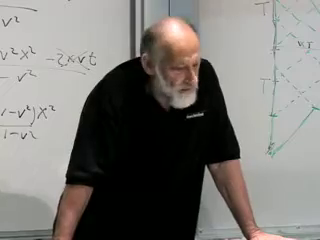
\includegraphics[width=0.72\textwidth]{lecture_04_figure_04.png}

\vspace{0.8em}

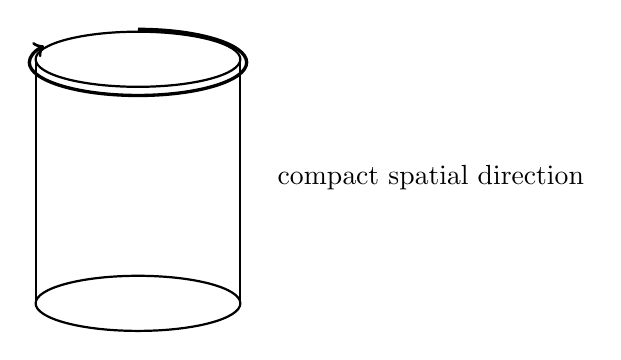
\begin{tikzpicture}[x=1cm,y=1cm]
\draw[thick] (0,0) ellipse (1.3 and 0.35);
\draw[thick] (-1.3,0) -- (-1.3,-3.1);
\draw[thick] (1.3,0) -- (1.3,-3.1);
\draw[thick] (0,-3.1) ellipse (1.3 and 0.35);
\draw[->,very thick] (0.0,0.38) arc (90:-210:1.38 and 0.42);
\node[right] at (1.65,-1.5) {compact spatial direction};
\end{tikzpicture}\caption{La cuestión del espacio compacto, tal como aparece en la pizarra, con un cilindro intrínseco bien definido. Se trata de una identificación global, no de un movimiento alrededor de un cilindro embebido en una dimensión radial adicional.}
\lectureframe{01:17:56}
\end{figure}

\section{La longitud se mide sobre una superficie de simultaneidad}

Ante un problema de relatividad especial, primero dibujemos el espacio-tiempo. Tomemos una regla de un metro en reposo en el sistema sin primas, con extremos en $x=0$ y $x=1$. A medida que pasa el tiempo, los dos extremos trazan líneas de universo verticales. La regla barre una cinta en el espacio-tiempo entre ellas.

El observador móvil debe medir ambos extremos en un mismo valor del tiempo móvil $t'$. Según la ec.~\eqref{eq:l4-simultaneity}, la superficie que pasa por el origen y cumple $t'=0$ satisface
\begin{equation}
t=vx
\end{equation}
en unidades de $c=1$. Esta superficie corta el extremo derecho $x=1$ en $t=v$.

\begin{figure}[H]
\centering
\includegraphics[width=0.73\textwidth]{lecture_04_figure_12.png}

\vspace{0.8em}

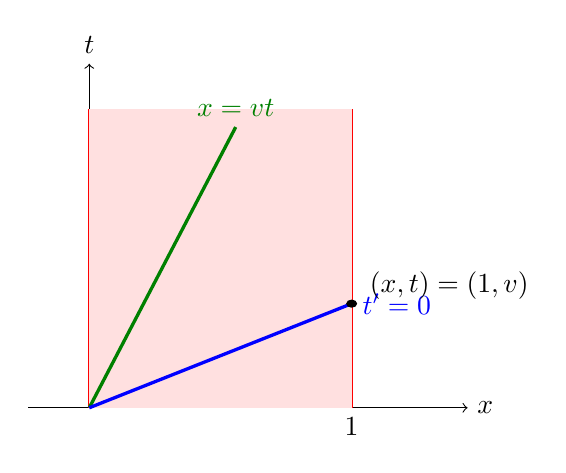
\begin{tikzpicture}[x=1.55cm,y=1.15cm]
\draw[->] (-0.5,0) -- (3.1,0) node[right] {$x$};
\draw[->] (0,0) -- (0,3.8) node[above] {$t$};
\draw[very thick,red] (0,0) -- (0,3.3);
\draw[very thick,red] (2.15,0) -- (2.15,3.3);
\fill[red!12] (0,0) rectangle (2.15,3.3);
\draw[very thick,green!50!black] (0,0) -- (1.2,3.1)
  node[above] {$x=vt$};
\draw[very thick,blue] (0,0) -- (2.15,1.15)
  node[right] {$t'=0$};
\fill (2.15,1.15) circle (0.045);
\node[right] at (2.22,1.35) {$(x,t)=(1,v)$};
\node[below] at (2.15,0) {$1$};
\end{tikzpicture}\caption{Una regla en reposo barre una cinta en el espacio-tiempo. La longitud medida por el observador móvil es la separación entre sus extremos sobre una superficie $t'=\mathrm{const}$.}
\lectureframe{01:24:20}
\end{figure}

La separación seleccionada entre los extremos es espacial, así que usamos la forma espacial positiva del invariante:
\begin{equation}
x'^2-t'^2=x^2-t^2.
\end{equation}
En el extremo elegido, $t'=0$, $x=1$ y $t=v$. Por tanto,
\begin{align}
x'^2&=1-v^2,\\
x'&=\sqrt{1-v^2}.
\end{align}
Así, en el sistema móvil, una longitud en reposo $L$ se mide como
\begin{equation}
L'=L\sqrt{1-v^2/c^2}=\frac{L}{\gamma}.
\label{eq:l4-length-contraction}
\end{equation}

\begin{figure}[H]
\centering
\includegraphics[width=0.76\textwidth]{lecture_04_figure_13.png}
\caption{La construcción completa de la contracción de la longitud y el resultado en la pizarra $x'=\sqrt{1-v^2}$ para una longitud en reposo unitaria.}
\lectureframe{01:28:10}
\end{figure}

También es cierta la afirmación recíproca: el observador del andén asigna una longitud menor a la regla longitudinal de un metro del tren. Una vez más, los dos observadores eligen sucesos simultáneos distintos para los extremos, de modo que la reciprocidad no es contradictoria.

\section{Preguntas finales}

\begin{classroomqa}\audiencequestion{¿Se propaga algo aparte de la luz a la velocidad de la luz? En particular, ¿qué ocurre con la gravedad?
\lecturetimestamp{01:29:29}}\lecturerresponse{La relatividad general predice ondas gravitacionales que se propagan a $c$. En la época de esta clase, las pruebas eran indirectas y provenían de sistemas como los púlsares binarios; todavía no se habían detectado ondas gravitacionales directamente.\editorialnote{La situación experimental cambió después de esta clase de 2006. LIGO detectó directamente GW150914 en 2015, y la observación conjunta de GW170817 y su contraparte electromagnética en 2017 mostró que las velocidades de propagación de la gravedad y de la luz coinciden con una diferencia de apenas unas pocas partes en $10^{15}$. Véanse \url{https://ligo.org/detections/gw150914/} y \url{https://doi.org/10.1103/PhysRevLett.119.251302}.}}
\end{classroomqa}

\begin{classroomqa}\audiencequestion{¿Puede un astronauta recorrer una distancia de muchos años luz en un tiempo propio menor que la distancia expresada en años luz? ¿Significaría eso que viaja más rápido que la luz?
\lecturetimestamp{01:30:38}}\lecturerresponse{El tiempo propio del astronauta es $\sqrt{\Delta t^2-\Delta x^2}$, menor que el tiempo coordenado $\Delta t$. En el sistema inercial del astronauta, la distancia entre las estrellas se contrae por Lorentz. Las estrellas se mueven con velocidad $-v$, no más rápido que la luz; simplemente hay menos distancia contraída que recorrer.}
\end{classroomqa}

Si el astronauta parte del reposo y acelera, la descripción cambia al pasar por una sucesión de sistemas inerciales instantáneos. La distancia asignada a las estrellas puede cambiar durante esa transición. No se puede aplicar una única transformación de Lorentz fija a toda la historia acelerada, pero el tiempo propio total sigue obteniéndose al sumar las contribuciones a lo largo de la línea de universo. Lo mismo vale para un gemelo realista que despega, gira y desacelera, en vez de nacer a velocidad de crucero.

\begin{classroomqa}\audiencequestion{¿Estos enigmas se deben a tratar el tiempo como algo especial? ¿Debemos llamarlo una cuarta dimensión?
\lecturetimestamp{01:36:43}}\lecturerresponse{No hace falta empezar con el eslogan de que el tiempo es una cuarta dimensión. La propia transformación de Lorentz obliga a que el espacio y el tiempo se mezclen, mientras que el intervalo $t^2-x^2-y^2-z^2$ los trata como partes de una misma geometría, con un signo distinto para el tiempo y el espacio. A bajas velocidades, la mezcla se vuelve despreciable y vuelve la intuición newtoniana habitual. Sin embargo, a velocidades relativistas, no se puede considerar que el espacio y el tiempo estén fundamentalmente desacoplados.}
\end{classroomqa}

Por tanto, la dilatación temporal, la contracción de la longitud, la comparación entre los gemelos y la reducción del tiempo de viaje no son trucos separados. Todo se desprende de tres hábitos: identificar los sucesos que se comparan, dibujar su geometría en el espacio-tiempo y usar el intervalo invariante.